\chapter{Supplement to ``Punctuated non-equilibrium and niche conservatism explain
  biodiversity fluctuations through the Phanerozoic''}

\section{Limit distribution of a time-averaged homogeneous
  origination-extinction process}
\label{sec:suppLimitDist}
Fossil taxa gain and lose taxa according to an origination-extinction
process. We assume that most fossil occurrences of a taxon come from
the period of its history when it is dominant and in steady state. In
a time slice of duration $\tau$ during such a period of steady state
the latent per capita rates of origination and extinction would be
equal (i.e. $\lambda = \mu \equiv \rho$) and the number of origination
or extinctions events (call such events $Y$) each follow an
inhomogeneous Poisson process with rate $\rho N_t$ where $N_t$ is the
number of species or genera in the taxon of interest at time
$t$. Allowing $N_t$ to vary smoothly with time, and invoking the
comunicative property of the Poisson distribution, we arrive at the
number $Y$ of extinction \emph{or} origination events in $\tau$ being
distributed
\begin{equation}
  \label{eq:eventPois1}
  Y \sim \text{Pois}(\rho \int_{t=0}^\tau N(t) dt).
\end{equation}
Under the steady state assumption we can approximate $N(t)$ by
$\bar{N}$, the steady state diversity, leading to
\begin{equation}
  \label{eq:eventPois2}
  Y \sim \text{Pois}(\rho \bar{N} \tau).
\end{equation}

Assuming the $\tau$ of each time period in the Paleobiology Database
or Sepkoski's compendium to be approximately equal (i.e. equal
durations of major stratographic units) then the distribution of
fluctuations within taxa will be asymptotically Gaussian.

\section{Additional super-statistical analyses}
To evaluate the sensitivity of our super-statistical analysis on the
particular data used and we tested our predictions on different data
sets (see below). The fact that it works in all different applications
indicates that it is robust to vagaries of different recording
strategies and bias corrections in paleobiology. This could mean that
much of the raw signal in massive fossil datasets, at least signals
regarding fluctuations, are not artifacts of sampling, as has been
proposed before \cite{hannisdal2011}.

\subsection{Raw PBDB data} \label{sec:rawPBDB}
We calculated the super-statistical prediction at the order level from
raw genus diversity recorded in the PBDB without correcting for
taphonomic or sampling bias (Fig. \ref{fig:supp_rawPBDB_Px}). The
super-statistical calculation also closely fits the raw data as in the
case of sampling and publication bias-corrected data.

\subsection{Different taxonomic ranks in PBDB data}
As noted in the main text, the super-statistical prediction
predictably breaks down at higher taxonomic scales. In Figure
\ref{fig:supp_PBDB_Px_cls} we present this worsening fit graphically
using class level data with three-timer and publication corrected PBDB
data

\subsection{Sepkoski's compendium} \label{sec:suppSepk}
Sepkoski's compendium \cite{sepkoski1992} provided the first
hypothesis of Phanerozoic diversification.  As such, it has served as
a benchmark for further investigation into large-scale paleobiological
patterns\cite{alroy08}.  We conducted the same super-statistical
analysis as in the main text and find comparable results.
Specifically, the super-statistical prediction far out preforms the
null Gaussian model (Fig. \ref{fig:supp_sepkPx}) and worsens with
increasing taxonomic scale (Fig. \ref{fig:supp_sepkPx}), again
implying the uniqueness of orders.

% \clearpage

% \bibliographystyle{pnas}
% \bibliography{../../bib/superStat}

\clearpage

\section*{Supplemental Figures}

\begin{figure}[!hp]
  \centering
%  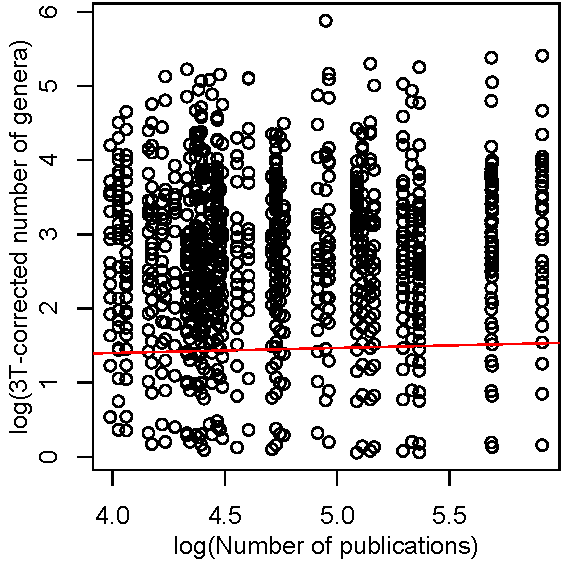
\includegraphics[scale=0.7]{figSupp_divByPub.pdf}
  \caption[Relationship between number of publications and genus
  diversity]{Relationship between number of publications and genus
    diversity as recorded by the PBDB.}
  \label{fig:divByPub}
\end{figure}

\begin{figure}[!hp]
  \centering
%  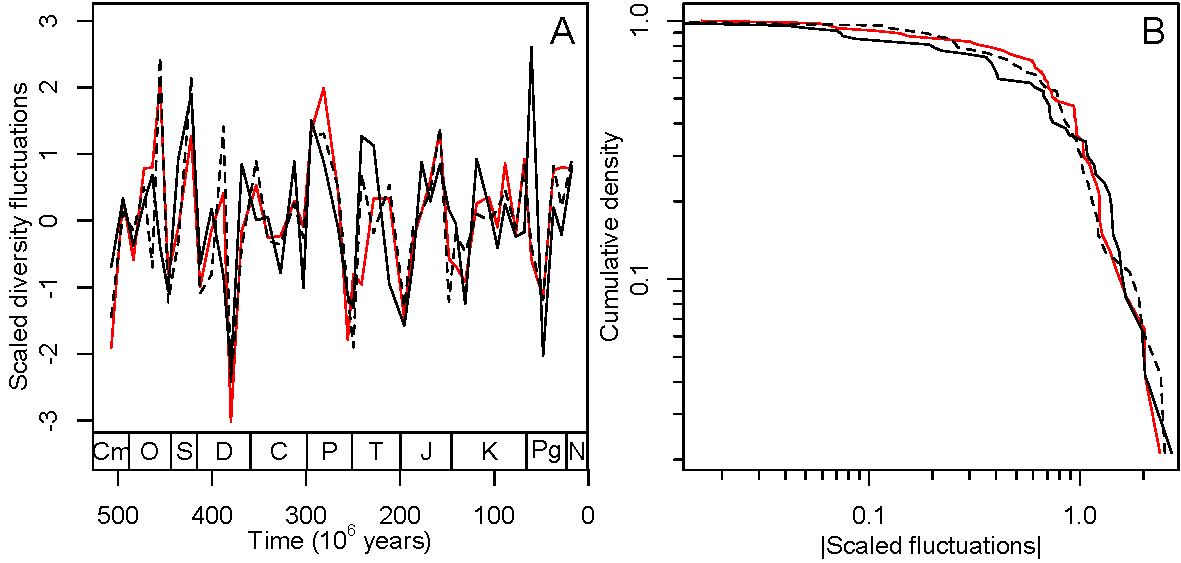
\includegraphics[scale=0.7]{figSupp_sqsRaw3tpub.pdf}
  \caption[Comparison of SQS method with the raw data and three-timer
  bias correction method]{Comparison of SQS method \cite{alroy2010}
    (solid black line) with the raw data (dashed black) and our
    three-timer and publication bias correction method (red). The
    time-series of all marine invertebrate genera shows general
    agreement with the only major deviations toward the modern
    (A). Despite these differences the distribution of fluctuations in
    genus diversity across all marine invertebrates show good
    agreement (B).}
  \label{fig:supp_3TPub}
\end{figure}

\begin{figure}[!hp]
  \centering
%  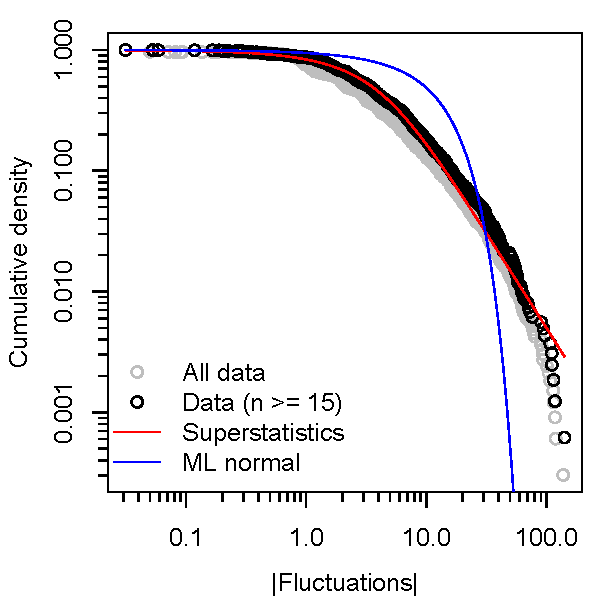
\includegraphics[scale=0.7]{figSupp_pbdbRaw_Px.pdf}
  \caption[Super-statistical prediction of raw data]{Super-statistical
    prediction of raw (i.e. not bias corrected) order-level
    fluctuations in genus diversity recorded in the PBDB. Grey dots
    are the full data of orders, while black ones are orders with more
    than 15 points. The red line is our theoretical prediction and the
    blue line the best Gaussian fit to the data.}
  \label{fig:supp_rawPBDB_Px}
\end{figure}

\begin{figure}[!hp]
  \centering
%  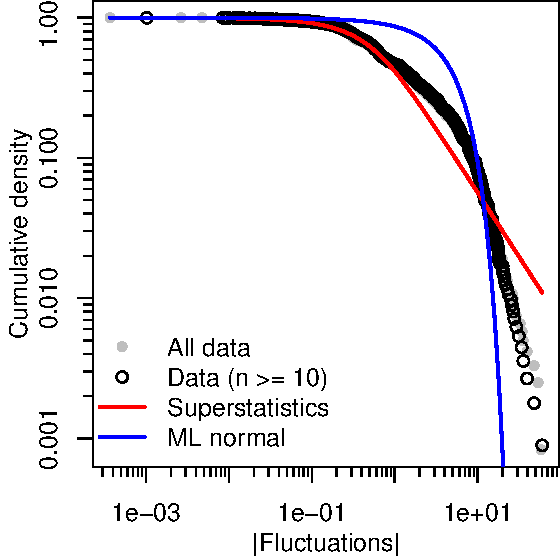
\includegraphics[scale=0.7]{figSupp_Px_cls.pdf}
  \caption[Super-statistical prediction of bias corrected class-level
  data]{Super-statistical prediction of bias corrected class-level
    fluctuations in genus diversity recorded in the PBDB. Grey dots
    are the full data of orders, while black ones are orders with more
    than 15 points. The red line is our theoretical prediction and the
    blue line the best Gaussian fit to the data. Note at the class
    level the fit is predictably worse, see main text for discussion.}
  \label{fig:supp_PBDB_Px_cls}
\end{figure}

\begin{figure}[!hp]
  \centering
%  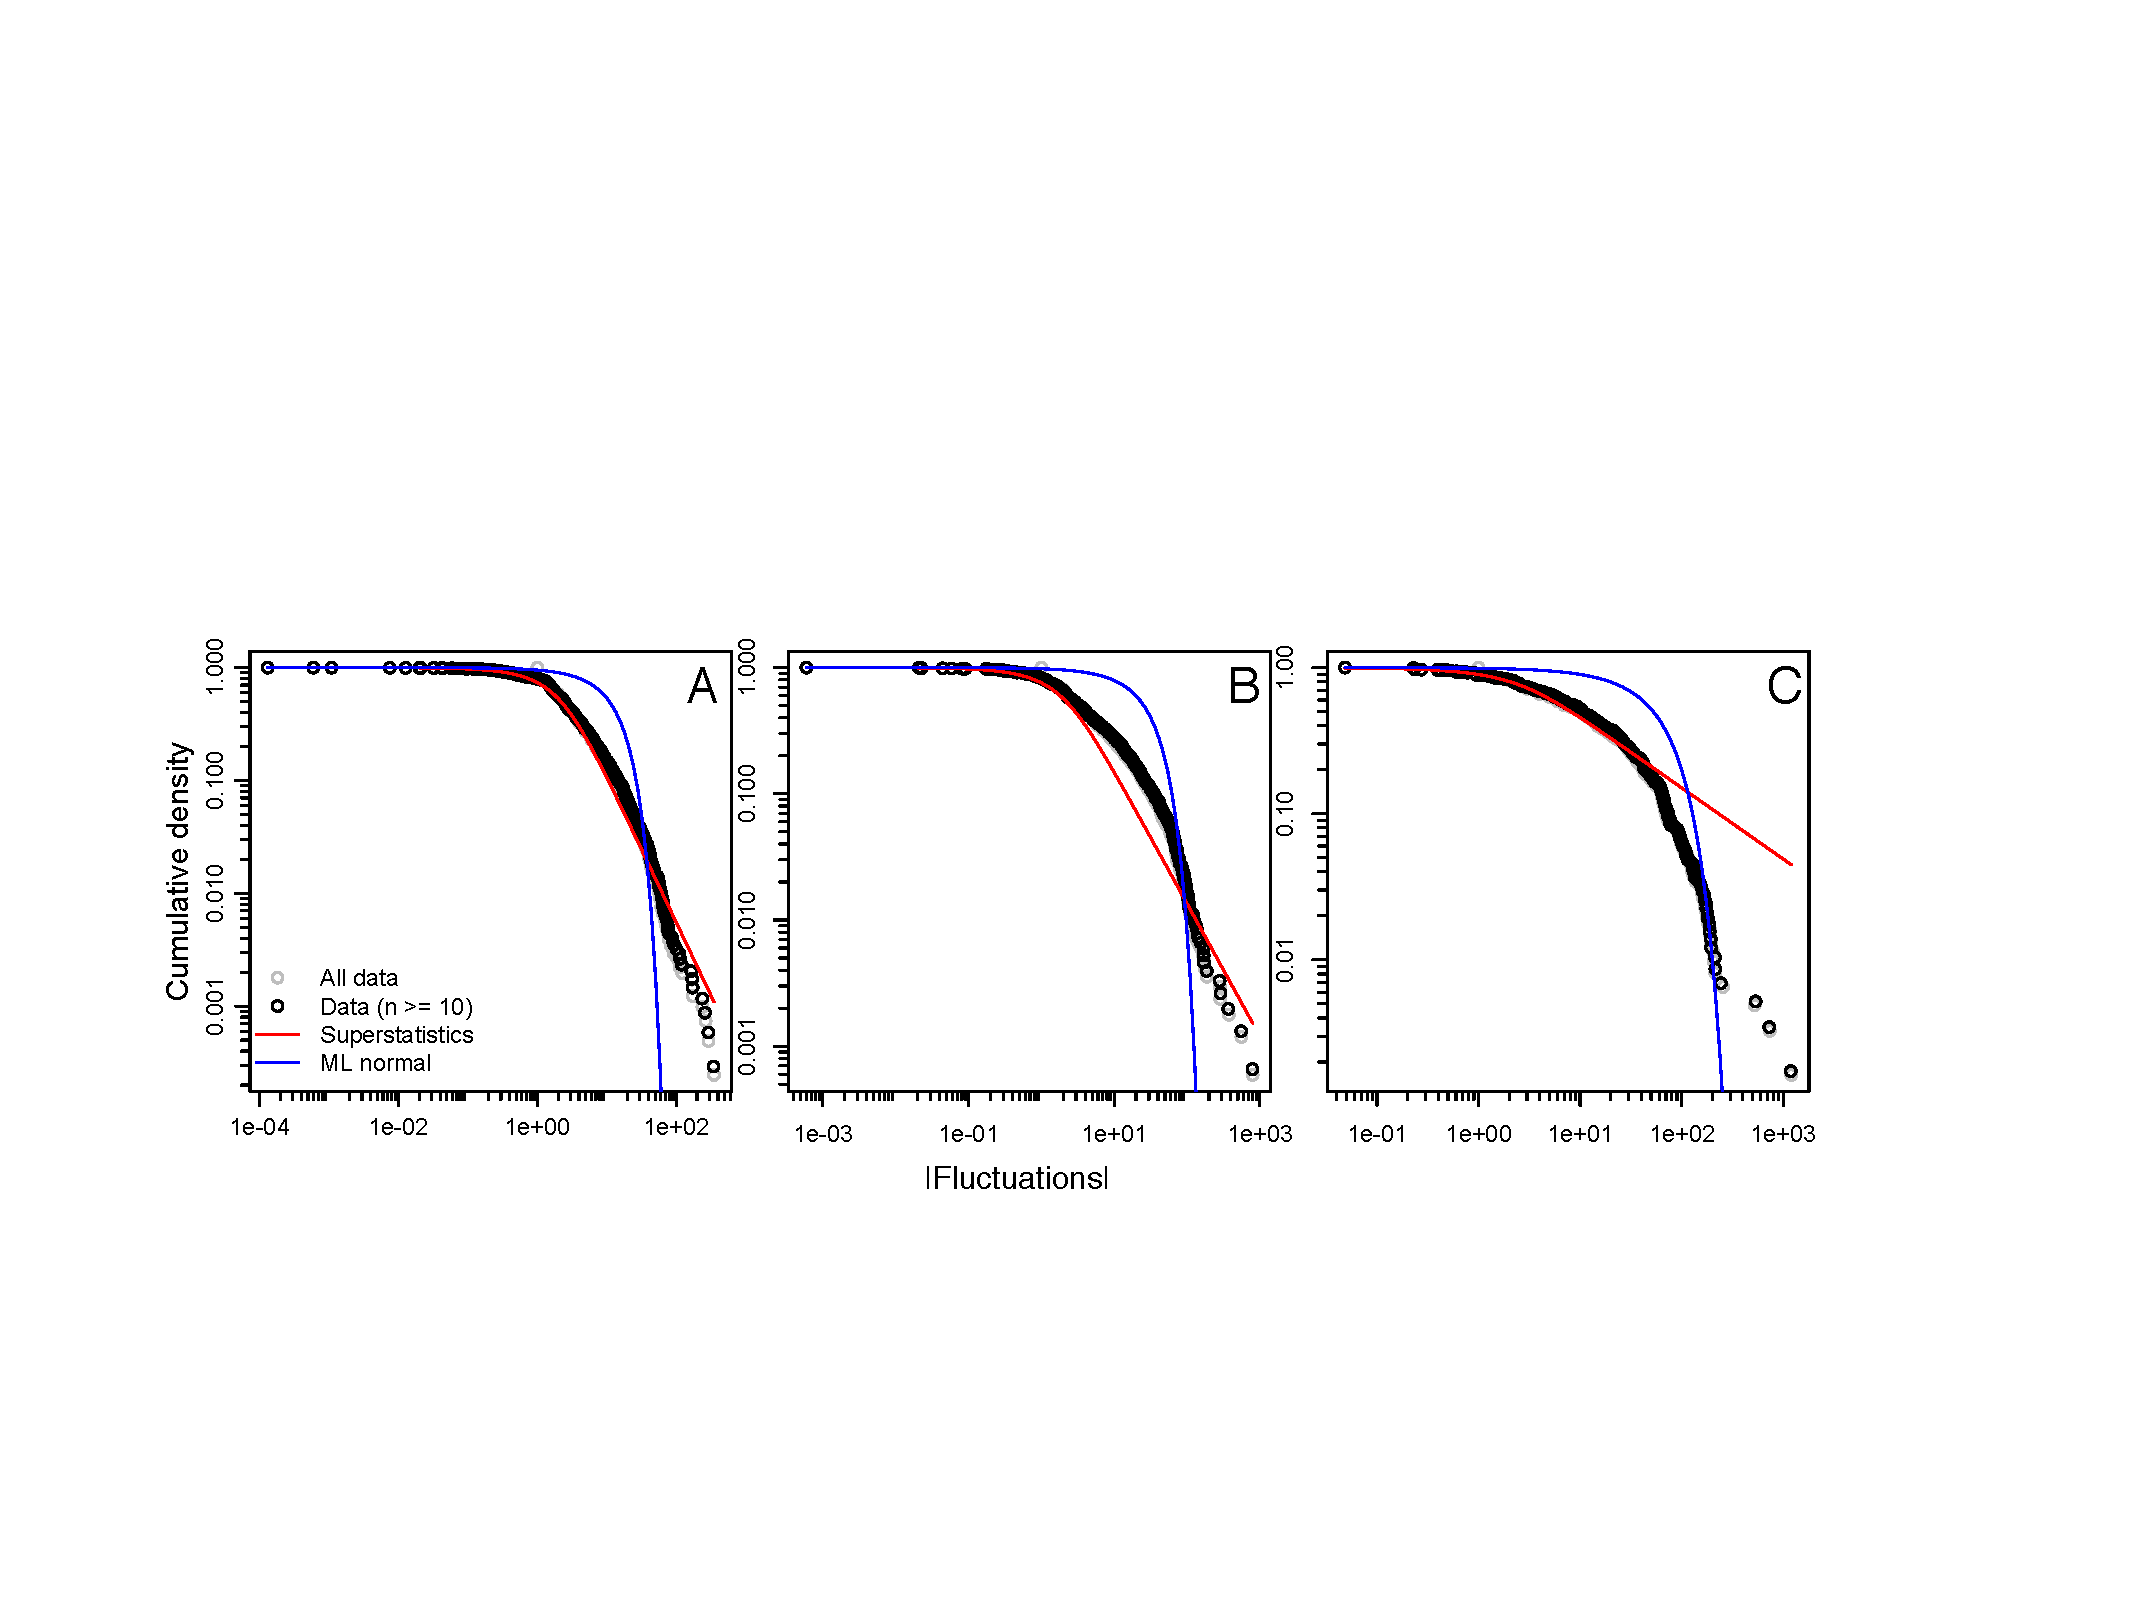
\includegraphics[scale=0.6]{figSupp_sepk_Px.pdf}
  \caption[Super-statistical prediction for Sepkoski's
  compendium]{Super-statistical prediction (red line) of fluctuations
    in genus diversity recorded in Sepkoski's compendium of marine
    invertebrates compared to maximum likelihood normal distribution
    (blue line). Super-statistical theory explains order level
    fluctuations well (A) with increasingly poorer fits at the class
    (B) and phylum (C) levels.}
  \label{fig:supp_sepkPx}
\end{figure}

